\documentclass[11pt,twoside,post]{octavo}

\usepackage[T1]{fontenc}
\usepackage[utf8]{inputenc}
\usepackage{mathpazo}
\usepackage{microtype}
\usepackage{amssymb}
\usepackage{xcolor}
\usepackage{tikz}
\usetikzlibrary{positioning,calc,shapes.geometric,backgrounds}
\usepackage[skins]{tcolorbox}
\usepackage{lettrine}
\usepackage{enumitem}

\definecolor{inkblue}{HTML}{1B2A4A}
\definecolor{claret}{HTML}{7A2E2E}
\definecolor{parchment}{HTML}{F3ECDD}
\definecolor{gilt}{HTML}{8B6B29}

\setcounter{secnumdepth}{1}
\setcounter{tocdepth}{1}

\renewcommand{\chaptername}{Essay}
\renewcommand{\thechapter}{\Roman{chapter}}

\color{inkblue}

\newcommand{\ornament}[1][1]{%
  \par\vspace{0.6em}
  \begin{center}
  \begin{tikzpicture}[baseline=0pt,scale=#1]
    \draw[claret,line width=0.5pt] (-1.6,0) -- (-0.32,0);
    \node[diamond,fill=gilt,draw=gilt,minimum size=5pt,inner sep=0pt] at (0,0) {};
    \draw[claret,line width=0.5pt] (0.32,0) -- (1.6,0);
  \end{tikzpicture}
  \end{center}
  \vspace{0.4em}\par
}

\newenvironment{pullquote}
  {\begin{tcolorbox}[
    colback=parchment,
    colframe=claret,
    boxrule=0.4pt,
    left=8pt,right=8pt,top=6pt,bottom=6pt,
    arc=0pt,
    fontupper=\itshape\small\color{inkblue}
  ]}
  {\end{tcolorbox}}

\setlist[itemize]{label={\color{claret}\small$\blacklozenge$},leftmargin=1.4em,itemsep=2pt,topsep=4pt}

\begin{document}

\frontmatter

\thispagestyle{empty}
\null\vspace{0.28\textheight}
\begin{center}
  {\Large \scshape Essays on a Quiet Craft}
\end{center}
\vfil\null
\cleardoublepage

\thispagestyle{empty}
\begin{center}
  \vspace*{2.2cm}
  {\huge \scshape Essays on \\[2pt] a Quiet Craft}\\[1.1em]
  \ornament[1.15]
  {\large\itshape Four Reflections on Attention, \\ Patience, and Work}
  \vfil

  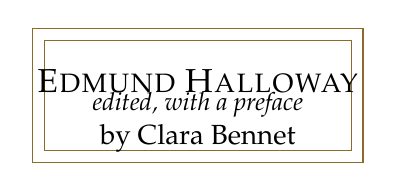
\begin{tikzpicture}
    \draw[gilt,line width=0.6pt] (-2.1,0.85) rectangle (2.1,-0.85);
    \draw[gilt,line width=0.3pt] (-1.95,0.7) rectangle (1.95,-0.7);
    \node at (0,0.18) {\large\scshape Edmund Halloway};
    \node[align=center] at (0,-0.34) {\small\itshape edited, with a preface\\ by Clara Bennet};
  \end{tikzpicture}

  \vfil
  {\scshape Meridian Press}\\
  {\small Aldermoor}
  \vspace{1.4cm}
\end{center}
\cleardoublepage

\thispagestyle{empty}
\vspace*{0.3\textheight}
\begin{center}
\begin{minipage}{0.82\textwidth}
\small
\textsc{Essays on a Quiet Craft}

\vspace{0.6em}
Copyright \copyright{} 2024 by the Estate of Edmund Halloway.

\vspace{0.6em}
First published in this edition by Meridian Press, Aldermoor. All rights reserved. No part of this publication may be reproduced, stored in a retrieval system, or transmitted in any form or by any means, electronic, mechanical, photocopying, or otherwise, without the prior written permission of the publisher, save for brief passages quoted in review.

\vspace{0.6em}
Typeset by the publisher in an antiqua letterform. Printed on acid-free paper.

\vspace{0.6em}
{\scshape Meridian Press} \\ Aldermoor
\end{minipage}
\end{center}
\cleardoublepage

\chapter{Editor's Preface}

\lettrine[lines=3,loversize=0.1,lraise=0.05]{T}{he four essays} gathered here were left, at the time of Edmund Halloway's death in the winter of 2022, in a single grey folder marked only \emph{for later, if ever}. He had spent forty years as a typesetter and, in his last decade, as a teacher of that trade to students who had never touched a composing stick. He did not think of himself as a writer. These pages suggest he was wrong.

What follows is not a treatise. Halloway distrusted treatises, and said so more than once at the long table in the Meridian Press workshop, usually with a proof sheet in one hand and a pencil in the other. The essays are occasional, written across some fifteen years, and they return again and again to a single question he never phrased quite the same way twice: what does it cost, and what does it earn, to do a slow thing well in a fast age?

I have changed almost nothing. Where a sentence trailed into the margin unfinished, I have finished it only when the sense was beyond doubt; where it was not, I have let it trail. Halloway believed an editor's chief duty was restraint. I have tried to honour that, even where it was inconvenient.

\begin{flushright}
\textit{C.\,B.}\\
\textit{Aldermoor}
\end{flushright}

\cleardoublepage

\thispagestyle{empty}
\vspace*{0.35\textheight}
\begin{center}
\textit{For the compositors,\\ who read every word\\ and are read by no one.}
\end{center}
\cleardoublepage

\thispagestyle{empty}
\vspace*{0.3\textheight}
\begin{center}
\begin{pullquote}
\begin{center}
The hand that hurries leaves a worse line than the eye can see at first, and a better one than the eye forgets.
\end{center}
\end{pullquote}

\vspace{0.8em}
\small --- from an undated marginal note, Halloway's workshop ledger
\end{center}
\cleardoublepage

\tableofcontents

\mainmatter

\chapter{On Attention as a Discipline}

\ornament

\lettrine[lines=3,loversize=0.1,lraise=0.05]{A}{ttention} is usually described as though it were a light one switches on: present or absent, on the page or wandering from it. I have come to think this is exactly backwards. Attention is not a lamp. It is a muscle, and like any muscle it is built by resistance, not by intention. You do not decide to have it. You earn it, one resisted distraction at a time, and you lose it the same way, one surrendered moment at a time.

I learned this at a composing frame, not a desk, which may be why I trust it more than I trust most things learned from books. Setting type by hand gives the attention nowhere to hide. Every character is a small physical decision, made at the speed of the hand rather than the speed of the thought, and the work simply stops if the mind leaves the room. A misplaced sort is not a metaphor. It sits in the forme, wrong, until someone notices.

\section*{The cost of the switch}

What the frame taught me, machines have since made easy to forget: that switching attention has a price, paid in full each time, whether or not the ledger shows it. A compositor who glances up at every noise in the shop does not merely lose the seconds of the glance. He loses the run-up, the small accumulated momentum by which a difficult line was about to resolve itself. He must build that momentum again from nothing. Do this often enough across a working day and you have not been interrupted twelve times; you have, in effect, started twelve short days and finished none of them.

\begin{pullquote}
The mind, unlike the hand, does not clock back in the moment you return to the bench. It arrives a little later, and a little poorer, each time.
\end{pullquote}

\ornament

\section*{A discipline, not a virtue}

I want to resist the temptation, common among people my age, to call sustained attention a lost virtue and leave it at that, as though the young were simply careless in a way we were not. It is not a virtue. Virtues are dispositions of character. Attention is closer to a trained skill, more akin to a straight cut than to honesty, and it responds to practice exactly as a straight cut does: badly at first, then less badly, then, if the practice holds, well enough that it looks effortless to anyone who has not tried it.

The discipline, such as it is, has one rule I have never found a way around. Decide in advance what you are attending to, before the temptation to attend to something else arrives, because no decision made in the moment of temptation is worth the paper it is not written on.

\chapter[Concerning Patience]{Concerning Patience in an Age of Speed}

\ornament

\lettrine[lines=3,loversize=0.1,lraise=0.05]{P}{atience} has an image problem. It is pictured as a kind of waiting room virtue, the discipline of the person who has nothing better to do, and so it loses, almost by default, every argument with speed, which is pictured as competence itself. I would like to make the case that this picture has the two exactly reversed, and that in most crafts worth practising, patience is the more aggressive of the two postures, not the more passive one.

Consider what a printer actually does when a forme will not lock up cleanly. The impatient response is to force it: more pressure on the quoins, a harder pull, a willingness to let a slightly crooked line stand because the alternative is to stop and find the true cause. The patient response is to stop, to pull the forme apart, and to look for the one furniture piece a hair's breadth out of true. This is not the slower option because the practitioner is calm. It is the slower option because it is doing more work, examining more of the problem, refusing to let the visible symptom stand in for the hidden cause.

\section*{Speed as a symptom}

I have started, in recent years, to treat any sudden increase in my own working speed as a symptom rather than an achievement, worth investigating rather than enjoying. Sometimes the increase is real and earned: the hand has finally learned the motion, and speed is simply what competence looks like from outside. But more often, in my experience, a sudden gain in speed means a corner has been found and is being cut, quietly, before the conscious mind has been informed.

\begin{pullquote}
Ask what you stopped checking, not what you started doing better.
\end{pullquote}

The distinction matters practically, because the two kinds of speed are almost indistinguishable from the inside and entirely distinguishable from the outside, usually about a week later.

\ornament

\lettrine[lines=2,loversize=0.05,lraise=0.02]{N}{one of this} is an argument for slowness as a general posture, which would be its own kind of affectation. It is an argument for a specific, narrow habit: treating patience as the default setting to be argued away from, rather than the exotic option to be argued toward, in any piece of work where the cost of a hidden error is higher than the cost of the extra hour spent looking for it.

\chapter[The Craftsman's Hand]{The Craftsman's Hand: Notes on Slow Work}

\ornament

\lettrine[lines=3,loversize=0.1,lraise=0.05]{E}{very trade} accumulates a small set of tools that are not, strictly, necessary, and that its practitioners nonetheless refuse to work without. In forty years at the bench I settled, eventually, on three. I offer them here not as equipment but as habits, since the tools were never really the point.

\begin{itemize}
  \item \textbf{A second pass, always, on a page you believe is finished.} Not a full re-reading, which the tired eye will only confirm rather than test, but a pass hunting one specific thing: widows, doubled words, a rule slightly out of alignment. The first pass tells you the work is done. The second tells you whether it is correct, and the two questions are less related than they appear.
  \item \textbf{A rule against composing the last hour of a long day.} The last hour is when a compositor is most confident and least reliable, a combination that has ruined more forms than fatigue alone ever did. Proofing, sorting, cleaning the case: these survive a tired hour. Setting new type rarely does.
  \item \textbf{A named place for every piece of unfinished work.} Not a pile. A place, with a name, that is checked on a schedule. A pile is where good intentions go to be forgotten in plain sight; a named, scheduled place is where they are merely delayed.
\end{itemize}

\section*{What the hand remembers}

There is a further habit I hesitate to recommend because it cannot quite be taught, only caught: trusting the hand's memory over the mind's judgment when the two disagree about a piece of familiar work. A hand that has set ten thousand ems of a particular face will hesitate, almost imperceptibly, over a sort that is subtly wrong in a way the eye has not yet consciously registered. I have learned, slowly and at some cost, to stop the hand and ask it why, rather than override it because the mind, in its haste, insists everything looks fine.

\begin{pullquote}
The hand is a slower reader than the eye, and a more honest one.
\end{pullquote}

\ornament

None of these notes amount to a method. A method could be written down entire and handed to a stranger. What I have described is closer to a set of manners: small, specific restraints that a craftsman imposes on himself, for reasons that were sound once and are worth re-examining periodically, but that mostly persist simply because abandoning them has always, in my experience, cost more than keeping them.

\chapter{On Reading Well}

\ornament

\lettrine[lines=3,loversize=0.1,lraise=0.05]{I}{ set type} for other people's sentences for most of my working life before I stopped to notice that I had never been taught, formally, how to read one. I had been taught to set it: to count its characters, to judge its measure, to notice where it would break awkwardly across a line. I had not been taught to read it, and I suspect this is more common than it sounds, since setting and reading feel so alike that it is easy to mistake long practice at one for competence at the other.

Reading well, as I have come to understand it late, is mostly a matter of speed discipline applied to the eye rather than the hand. The fast reader extracts the gist of a sentence and moves on, which is a perfectly reasonable strategy for most of what crosses a desk in a day. It becomes a poor strategy exactly at the point where a sentence has been built carefully enough that its gist is not the same as its meaning, and a good sentence, in my trade's oldest sense of good, very often has exactly this structure: a plain surface with a further claim folded underneath it.

\section*{A compositor's test}

I still use a test from the composing room, adapted. A compositor checks a difficult line by reading it backward, word by word, because the ordinary forward reading is too fluent to catch a small error; the mind fills gaps the backward reading will not permit it to fill. I have found a version of this useful for prose meant to be believed rather than merely understood: read the argument once forward for the pleasure of it, and once more, deliberately, hunting for the sentence doing the least obvious work. It is usually there for a reason.

\begin{pullquote}
A sentence that asks nothing of you was very likely written by someone who asked nothing of himself.
\end{pullquote}

\ornament

I do not offer this as a general theory of reading, only as the one habit that has most repaid the trouble of keeping it, from a trade that spent most of its energy on the setting of words and, only very late, on their reading.

\backmatter

\chapter{A Note on the Type}

This edition follows the house convention at Meridian Press of setting essay collections in a modern revival of the old antiqua letterforms: the roman hand that displaced blackletter in the printing shops of southern Europe and, over several centuries, became simply what most readers mean when they picture a printed page. The name persists mainly by contrast, a reminder that the shape of a letter was once a live argument rather than a settled default.

The present text is composed with generous margins and a narrow measure, following the classical page canons by which the proportion of a book's type block was fixed to the proportion of its leaf, rather than to the convenience of a particular press. Halloway, who set type for a living and read about it for pleasure, would probably have found this note longer than it needed to be. It is kept here anyway, on the theory that a book about slow, deliberate craft ought to say plainly what has been done to make its own pages.

\chapter{About the Author}

Edmund Halloway (1911--2022) trained as a compositor at Meridian Press in his early twenties and remained associated with the house, in one capacity or another, for the rest of his working life. He was, by his own account, an indifferent apprentice and a stubborn journeyman, and he took evident pride in having become, eventually, a patient teacher of a trade that by the end of his career very few people still practised by hand.

He is survived by several generations of typesetters who passed through his workshop, a number of unfinished manuscripts, and the four essays collected in this volume, which he was persuaded, more than once and without success, to publish during his lifetime.

\end{document}
